\begin{figure*}[ht]
    \vspace{-10pt}
    \begin{minipage}[b]{\textwidth}
        % \begin{center}

        \subfigure[aligned MHC pangenome]{
            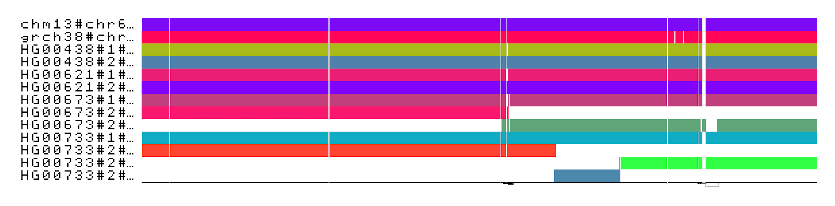
\includegraphics[width=.48\textwidth]{fig/mhc-align.eps}
            \label{fig:1a}
        }
        \vspace{-11pt}
        % \newline
        \subfigure[consensus MHC pangenome]{
            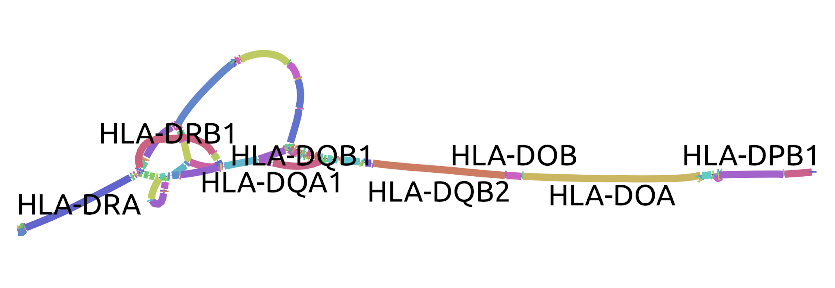
\includegraphics[width=.48\textwidth]{fig/mhc-pangenome.eps}
            \label{fig:1b}
        }
        \caption{Pangenome visualisations of the Major Histocompatibility Complex (MHC) \textit{locus} by \odgi.
            (a) projection of full MHC \textit{locus} of haploid phased human genome
          assemblies, plus the chm13 cell line and GRCh38 reference genome (note the missing patch in the reference
          genome) as supplied by the
            Human Reference Pangenome Consortium\citep{HRPC} and created by \cmd{odgi build+sort+viz}. The coloured
            bars represent the linearised paths --- representing contigs as a zoomed out multi-sequence
            alignment.
            (b) consensus graph representation by \cmd{odgi build} of the same assemblies showing variations larger than $100$ base pairs.
            Loops or `bubbles' display contigs uniquely diverging from the consensus, caused by variation in repeats.
            The gene labels are super imposed by \cmd{odgi position} from a GRCh38 BED file and visualised by the Bandage tool\citep{26099265}.
        }
        \label{fig:1}
        % \end{center}
    \end{minipage}
\end{figure*}
